
\documentclass[11pt,a4paper]{article}

% ---- Packages ----
\usepackage[utf8]{inputenc}
\usepackage[T1]{fontenc}
\usepackage{mathpazo}
\usepackage{amsmath,amssymb}
\usepackage{graphicx}
\usepackage{booktabs}
\usepackage{longtable}
\usepackage{float}
\usepackage{geometry}
\usepackage{setspace}
\usepackage{xcolor}
\usepackage[
  colorlinks=true,
  linkcolor={blue!70!black},
  citecolor={red!60!black},
  urlcolor={teal!80!black}
]{hyperref}
\usepackage{caption}
\usepackage{lineno}

% ---- Page layout ----
\geometry{margin=2.5cm}
\onehalfspacing
\setlength{\parindent}{0pt}
\setlength{\parskip}{6pt plus 2pt minus 1pt}

% ---- Font sizes ----
\captionsetup{font=small, labelfont=bf}

% ---- Pandoc compat ----
\providecommand{\tightlist}{\setlength{\itemsep}{0pt}\setlength{\parskip}{0pt}}

% ---- Section font sizes ----
\usepackage{titlesec}
\titleformat{\section}{\large\bfseries}{\thesection}{1em}{}
\titleformat{\subsection}{\normalsize\bfseries}{\thesubsection}{1em}{}
\titleformat{\subsubsection}{\normalsize\itshape}{\thesubsubsection}{1em}{}
\titleformat{\paragraph}[runin]{\normalsize\bfseries}{\theparagraph}{1em}{}[.]

% ============================================================
\title{\Large A Modular Framework for Enhancing Satellite-Derived Daily
Precipitation:\\[4pt]
Adjusting Values, Aligning Distributions, and Preserving Extremes\\[8pt]
\normalsize\textit{Seminar Draft}}

\author{\normalsize
Benny Istanto\textsuperscript{1,*} \and
Rizaldi Boer\textsuperscript{2,3} \and
I Putu Santikayasa\textsuperscript{2,4}
}

\date{\small
\textsuperscript{1} Applied Climatology Study Program, Department of Geophysics and Meteorology,\\
Bogor Agricultural University, Bogor 16680, Indonesia\\[2pt]
\textsuperscript{2} Department of Geophysics and Meteorology, Bogor Agricultural University, Bogor 16680, Indonesia\\[2pt]
\textsuperscript{3} International Research Institute for Environment and Climate Change,\\
Bogor Agricultural University, Bogor 16680, Indonesia\\[2pt]
\textsuperscript{4} Center for Climate Risk and Opportunity Management in South East Asia and Pacific,\\
Bogor Agricultural University, Bogor 16680, Indonesia\\[6pt]
* Correspondence: bennyistanto@gmail.com
}

\begin{document}
\linenumbers
\maketitle

% ============================================================
\begin{abstract}
Accurate daily precipitation estimates are essential for hydrological
modeling, climate risk assessment, and disaster preparedness.
Satellite-based products such as IMERG provide global coverage but
exhibit systematic biases in daily accumulations, particularly in
representing extreme precipitation events. This study presents a hybrid
bias correction framework (LSEQM+DL) that sequentially integrates
Linear Scaling (LS), Empirical Quantile Mapping (EQM) with Generalized
Pareto Distribution (GPD) tail adjustment, and Convolutional Neural
Network (CNN) refinement. A station density confidence mask modulates
CNN influence based on gauge network density. Applied to daily IMERG
Late Run over Indonesia (2001--2025) and evaluated against 171
independent BMKG station observations, the framework brings the standard
deviation ratio from 0.71 (LS) to 1.00 (LSEQM+DL), the relative bias
from \(-\)11.4\% to \(-\)0.6\%, and the 99th-percentile ratio from 0.71
to 1.01. The wet-day frequency ratio improves from 1.21 to 0.95,
reducing a 21\% overestimation of wet-day occurrence to within 5\% of
observed. Event detection (POD) decreases from 0.78 to 0.65, reflecting
the trade-off inherent to distributional correction. WMO multi-threshold
verification confirms maintained skill at thresholds up to 100~mm/day.
The framework relies on globally available datasets and is applicable
to other tropical regions with sparse gauge networks.
\end{abstract}

\noindent\textbf{Keywords:} Bias Correction; Satellite Precipitation;
IMERG; Extreme Events; Deep Learning; Quantile Mapping; Generalized
Pareto Distribution; Quality Assessment; Indonesia

% ============================================================
\section{Introduction}\label{introduction}

Accurate daily precipitation estimates underpin flood forecasting,
agricultural planning, hydrological modeling, and climate risk
assessment. Satellite-based products such as the Integrated
Multi-satellitE Retrievals for Global Precipitation Measurement (IMERG)
provide near-global coverage \cite{ref1,ref2} but exhibit systematic biases
relative to surface observations: overestimation of light-rain days,
underestimation of heavy events, and distributional mismatch that
degrades the representation of extremes \cite{ref3}. These limitations are
particularly consequential in tropical regions such as Indonesia, where
convective rainfall dominates and ground gauge networks are sparse.

Several bias correction approaches address different aspects of this
problem. Linear Scaling (LS) removes the mean bias but leaves the
distribution shape unchanged \cite{ref4}. Empirical Quantile Mapping (EQM)
aligns the full distribution but can underrepresent the upper tail
\cite{ref5,ref6}. Generalized Pareto Distribution (GPD) fitting targets
extreme values explicitly \cite{ref7} but is typically applied in isolation.
Convolutional Neural Networks (CNNs) capture spatially complex residual
patterns \cite{ref9,ref10} but risk overfitting in data-sparse regions.
No prior study has integrated all four components into a sequential,
physically interpretable framework for daily satellite precipitation
correction.

This paper presents LSEQM+DL, a hybrid framework that addresses mean
bias, distributional alignment, and extreme event preservation in
sequence. Applied to daily IMERG Late Run over Indonesia (2001--2025)
and validated against CPC-UNI gridded observations \cite{ref13} and 171
independent BMKG station records, the framework yields substantial,
independently verified improvements. The three design objectives provide
the organizing structure for both the methods and the evaluation:
\emph{adjusting values}, \emph{aligning distributions}, and
\emph{preserving extremes}.

% ============================================================
\section{Study Region, Data, and Methods}\label{methods}

\subsection{Study Region}

Indonesia (95--141\textdegree E, 11\textdegree S--6\textdegree N) is the
world's largest archipelago, presenting a complex precipitation
environment: a trimodal rainfall regime driven by the monsoon and
Maritime Continent convective cycle \cite{ref19,ref20}, frequent extreme
events, and a gauge network heavily concentrated in Java and southern
Sumatra. The 180 CPC-UNI contributing stations provide adequate
constraint in western Indonesia but sparse coverage over Papua, Maluku,
and eastern Nusa Tenggara. This spatial heterogeneity provides both a
demanding test environment and a practical motivation for the station
density confidence mask (Section~\ref{sec:stage4}).

\subsection{Datasets}

Three precipitation datasets are used. IMERG Late Run (IMERG-L;
0.1\textdegree, $\sim$14-hour latency) \cite{ref2,ref21} is the product to
be corrected; because it relies purely on satellite observations without
gauge assimilation, it provides an uncontaminated baseline. IMERG Final
Run (IMERG-F; 0.1\textdegree) \cite{ref2}, which incorporates gauge data
during post-processing, is included as an independent benchmark. CPC
Unified Gauge-Based Analysis of Daily Precipitation (CPC-UNI;
0.5\textdegree) \cite{ref13,ref18} is the correction reference. Independent
validation uses 171 BMKG stations with at least 30 valid daily records
per dekadal period (Figure~\ref{fig:stations}).

Preprocessing harmonizes all datasets through nearest-neighbor
regridding, temporal alignment, land-sea masking, and latitude
reindexing. Following the Bias Correction Spatial Disaggregation (BCSD)
principle \cite{ref23}, distribution parameters are estimated at the native
0.5\textdegree{} CPC-UNI resolution and interpolated to 0.1\textdegree{}
before quantile mapping is applied. A wet-day threshold of 1.0~mm/day is
applied throughout \cite{ref24}.

\subsection{Hybrid Bias Correction Framework}

The framework corrects daily satellite precipitation through four
sequential stages, each targeting a distinct source of systematic bias
(Figure~\ref{fig:framework}). Processing is performed independently for
each of 36 dekadal windows (three 10-day periods per month), with
statistics pooled across all years (approximately 230 samples per
dekad) for robust distribution fitting.

\begin{figure}[H]
\centering
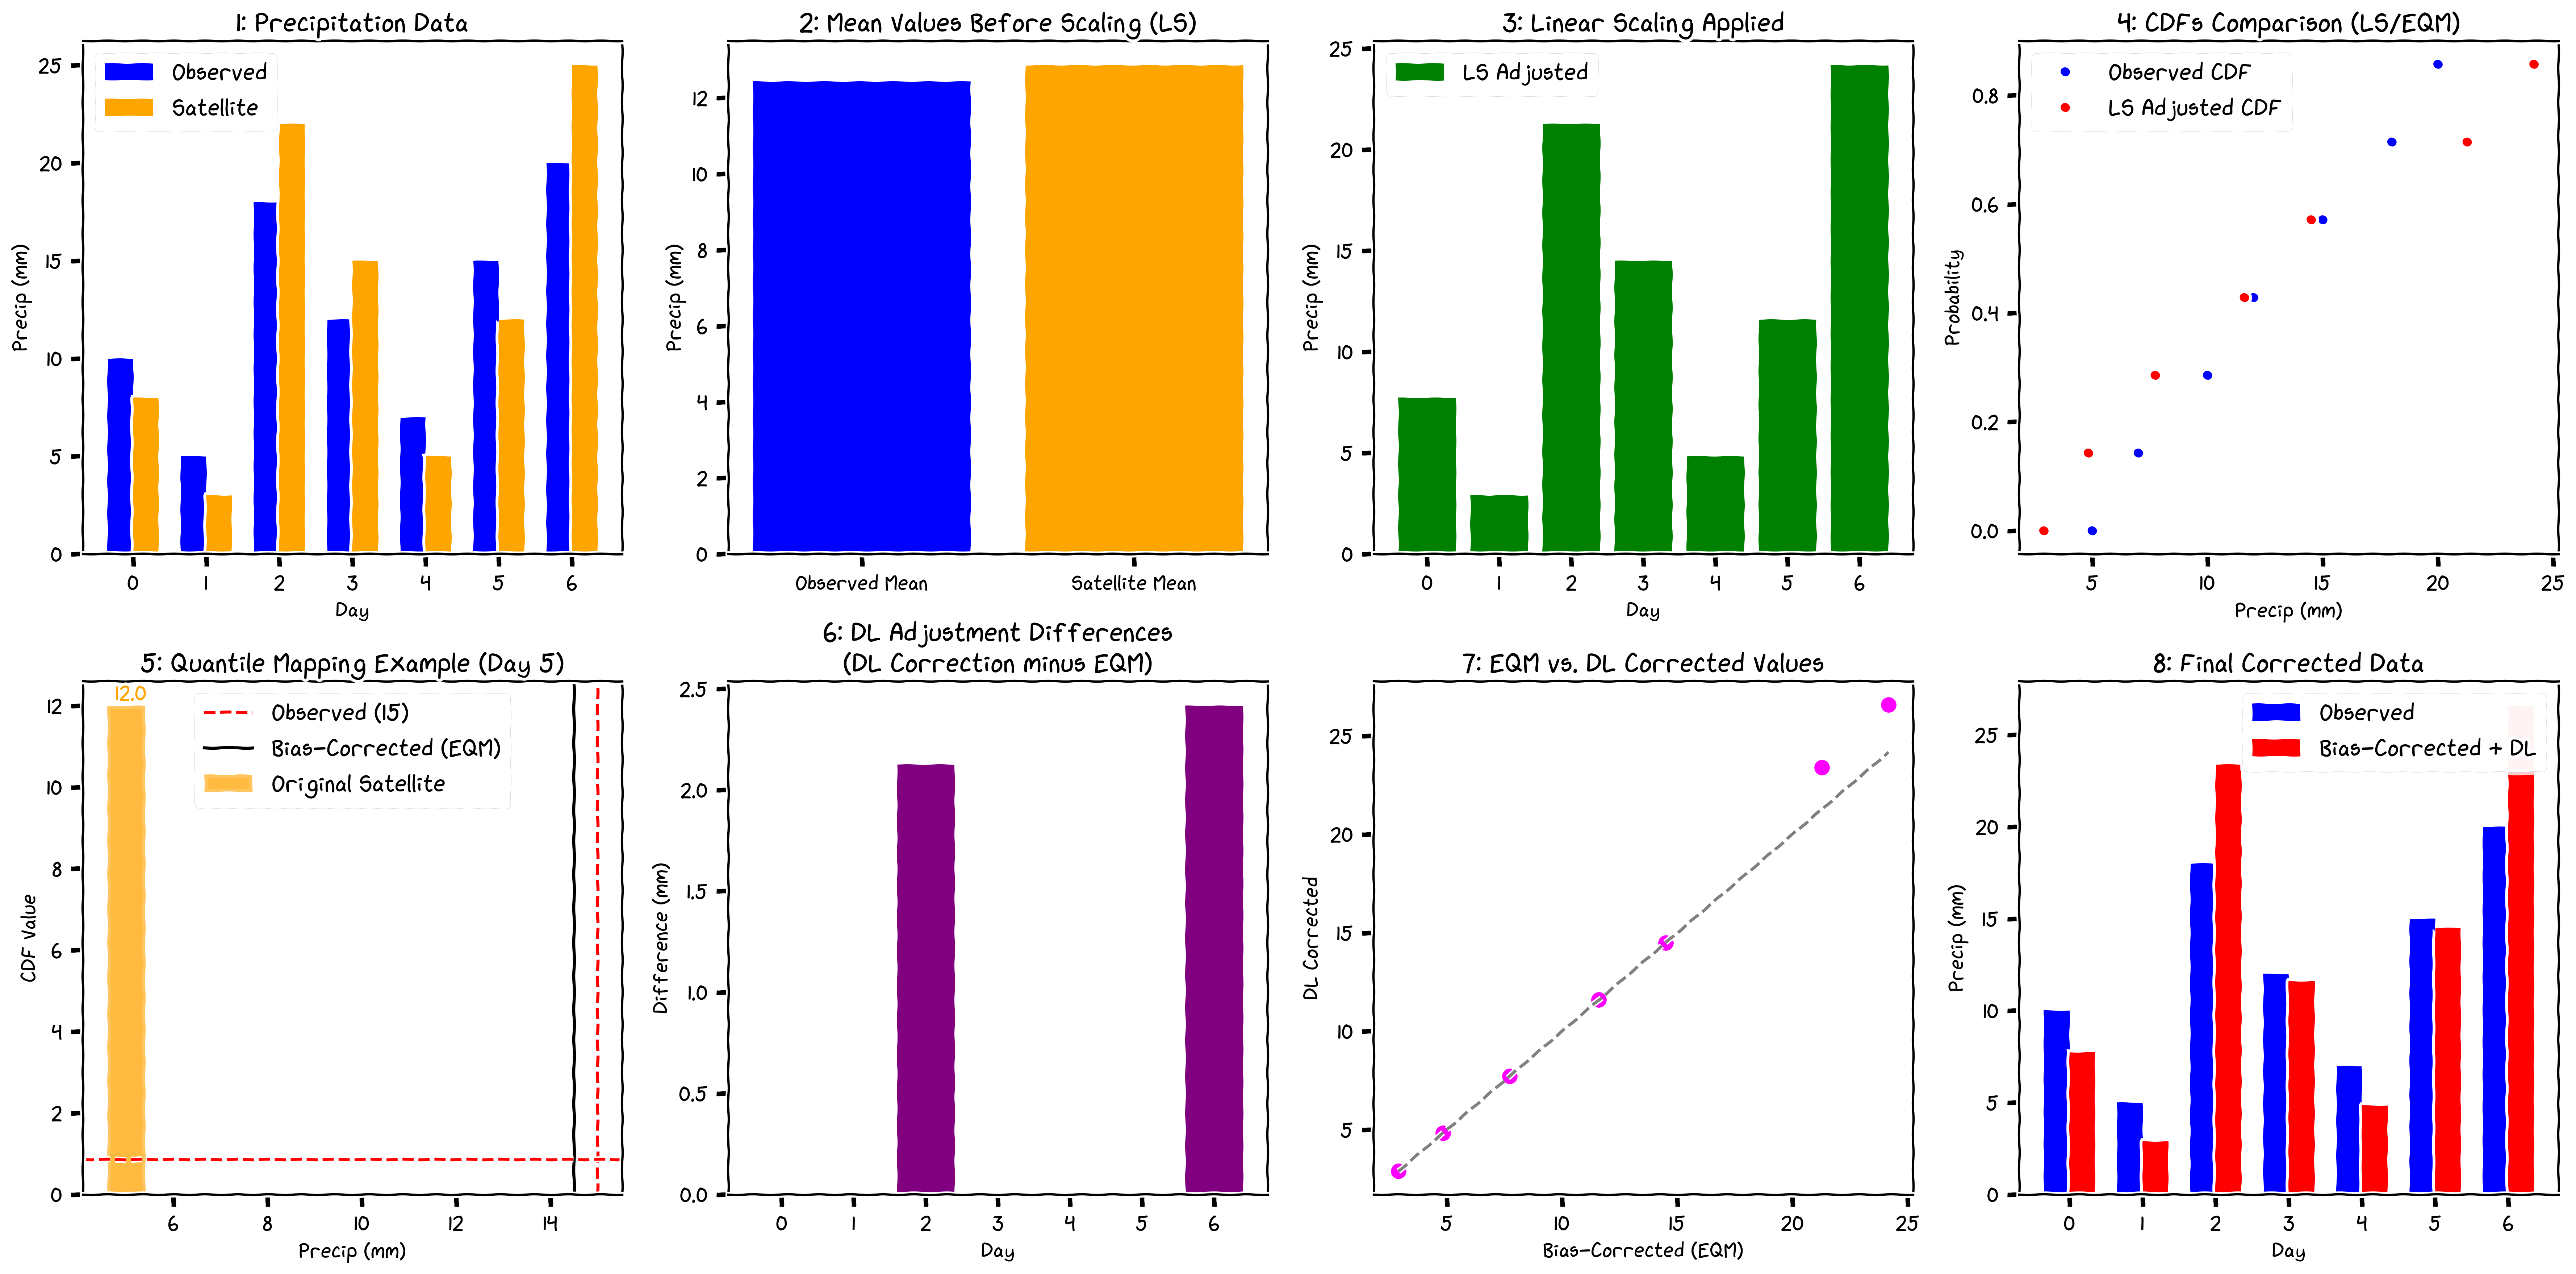
\includegraphics[width=0.65\textwidth]{images/fig01_framework.png}
\caption{Conceptual workflow of the LSEQM+DL hybrid bias correction
framework.\label{fig:framework}}
\end{figure}

\subsubsection{Stage 1: Linear Scaling}

Linear Scaling removes the mean bias by multiplying each satellite field
by a dekad-specific factor:

\begin{equation}
C_{LS} = \frac{\bar{P}_{ref}}{\bar{P}_{sat}},
\qquad
P_{LS} = P_{sat} \cdot C_{LS}
\label{eq:ls}
\end{equation}

where $\bar{P}_{ref}$ and $\bar{P}_{sat}$ are the dekadal mean daily
precipitation of CPC-UNI and IMERG-L, respectively. The scaling factor
is computed at the native 0.5\textdegree{} CPC-UNI resolution and
bilinearly interpolated to 0.1\textdegree{}, producing a spatially smooth
correction field \cite{ref23}.

\subsubsection{Stage 2: Empirical Quantile Mapping (EQM)}

Empirical Quantile Mapping aligns the full cumulative distribution
function (CDF) of the LS-corrected field to that of the reference.
Gamma distributions are fitted to the wet-day sample using maximum
likelihood estimation \cite{ref15}, and the quantile correction is:

\begin{equation}
P_{EQM} = F_{ref}^{-1}\!\left(F_{sat}(P_{LS})\right)
\label{eq:eqm}
\end{equation}

where $F_{sat}$ and $F_{ref}$ are the fitted satellite and reference
gamma CDFs, respectively. Dry-day handling follows Cannon et
al.~\cite{ref11}, preserving the reference dry-day frequency by
construction and preventing satellite drizzle from mapping to spurious
low-intensity wet-day values.

\subsubsection{Stage 3: GPD Tail Adjustment}

Gamma-based EQM can underrepresent the upper tail of the precipitation
distribution. Exceedances above the 80th percentile of the wet-day
sample are instead modeled with the Generalized Pareto Distribution
\cite{ref7}. For an LS-corrected value $P_{LS}$ exceeding the satellite
threshold $u_{sat}$, the conditional exceedance probability and
GPD-corrected value are:

\begin{equation}
p_c = \frac{F_{sat}(P_{LS}) - F_{sat}(u_{sat})}{1 - F_{sat}(u_{sat})},
\qquad
P_{LSEQM} = u_{ref} + G_{ref}^{-1}(p_c)
\label{eq:gpd}
\end{equation}

where $G_{ref}^{-1}$ is the inverse GPD fitted to the reference
exceedances and $u_{ref}$ is the reference 80th percentile. GPD
parameters are estimated at 0.5\textdegree{} and interpolated to
0.1\textdegree{}. Corrected values are capped at the interpolated
99.9th percentile of the reference distribution to prevent physically
unrealistic extrapolation.

\subsubsection{Stage 4: CNN Refinement and Spatial Modulation}
\label{sec:stage4}

Residual biases in extreme precipitation pixels, arising from complex
spatial patterns that statistical methods cannot capture, are addressed
by a CNN trained separately for each dekadal period with LSEQM-corrected
fields as input and CPC-UNI as the training target. CNN corrections are
applied selectively to extreme pixels through alpha-blending:

\begin{equation}
P_{final} = \alpha_{eff} \cdot P_{LSEQM} + (1 - \alpha_{eff}) \cdot P_{DL}
\label{eq:blend}
\end{equation}

applied only to pixels where $P_{LSEQM}$ exceeds the 80th percentile of
the dekadal distribution; non-extreme pixels retain their LSEQM values.
The effective blending weight is modulated by a station density
confidence mask $C(x,y) \in [0,1]$:

\begin{equation}
\alpha_{eff}(x,y) = 1.0 - C(x,y) \cdot (1.0 - \alpha)
\label{eq:mask}
\end{equation}

where $\alpha = 0.70$ is the base weight. The confidence mask is derived
from gauge counts per 0.5\textdegree{} cell, Gaussian-smoothed to
prevent sharp boundaries, and normalized by a saturation count of 3
stations. Station-dense areas receive the full CNN contribution
($\alpha_{eff} = 0.70$); station-sparse areas revert toward pure LSEQM
($\alpha_{eff} \to 1.0$) \cite{ref27}.

\subsection{Evaluation Approach}

Performance is assessed through 31 pixel-level metrics organized by
three evaluation pillars aligned with the design objectives: value
adjustment (relative bias, standard deviation ratio), distribution
alignment (Kolmogorov-Smirnov test, wet-day frequency ratio, wet-day
intensity ratio, six percentile ratios), and extreme preservation
(95th- and 99th-percentile ratios, WMO multi-threshold verification at
seven thresholds from 1 to 150~mm/day). A Composite Quality Index (CQI)
integrates these metrics into a single score on $[0,1]$.

Evaluation employs two reference datasets: CPC-UNI (the correction
target, for domain-wide assessment) and 171 independent BMKG station
observations not used in the correction procedure (for ground truth
validation). This two-reference design distinguishes genuine
improvements from overfitting to the training reference.

% ============================================================
\section{Results}\label{results}

\subsection{Domain-wide Performance}\label{sec:domain}

Table~1 summarizes the domain-wide spatial median across
all land pixels. Linear Scaling reduces the relative bias against CPC-UNI
to zero by construction, but the standard deviation ratio of 0.971
confirms that uniform multiplicative rescaling leaves the distribution
shape essentially unchanged. The LSEQM stage reshapes the distribution:
the wet-day-mean ratio increases from 0.961 to 1.157, the $Q_{99}$ ratio
from 0.967 to 1.212, and the wet-day frequency ratio decreases from 1.040
toward 0.947. The apparent overshoot of upper percentile ratios above
unity against CPC-UNI reflects a conditional bias in the gridded
reference rather than over-correction; independent station validation
(Section~\ref{sec:station}) confirms ratios near 1.0 against gauges.
Event detection shows a modest trade-off: POD decreases from 0.767 to
0.707 as dry-day frequency matching reclassifies some satellite wet days,
while FAR improves from 0.271 to 0.248. Temporal accuracy metrics
(Pearson correlation, RMSE, NSE) remain essentially unchanged, consistent
with the theoretical constraint that quantile mapping adjusts marginal
distributions without modifying temporal sequencing \cite{ref34}.

\phantomsection\label{tab:domain}
\textbf{Table~1.} Domain-wide evaluation by correction stage against
CPC-UNI. Values represent the spatial median across all land pixels.
Ratio metrics express test/reference (target = 1.0). Bold indicates the
value closest to the target.

\begingroup\small
\begin{longtable}[]{@{}llllll@{}}
\toprule
Evaluation Objective & Metric & LS & LSEQM & LSEQM+DL & Target \\
\midrule
\endhead
\bottomrule
\endlastfoot
\textbf{Value Adjustment}
  & Relative Bias        & \textbf{0.0000} & 0.0697 & 0.0652 & 0 \\
  & Std.\ Dev.\ Ratio    & 0.9707 & 1.1587 & 1.1475 & 1.0 \\
\textbf{Distribution Alignment}
  & KS \(p\)-value (\%) & 6.56 & 0.00 & 0.00 & 100 \\
  & Wet-Day Freq.\ Ratio & \textbf{1.0397} & 0.9466 & 0.9462 & 1.0 \\
  & Wet-Day Int.\ Ratio  & 0.9611 & \textbf{1.1569} & 1.1519 & 1.0 \\
\textbf{Extreme Preservation}
  & \(Q_{95}\) Ratio     & 0.9459 & 1.1711 & \textbf{1.1626} & 1.0 \\
  & \(Q_{99}\) Ratio     & 0.9669 & 1.2117 & \textbf{1.1964} & 1.0 \\
\textbf{Event Detection}
  & POD                  & \textbf{0.7669} & 0.7069 & 0.7069 & 1.0 \\
  & CSI                  & \textbf{0.5890} & 0.5723 & 0.5724 & 1.0 \\
  & FAR                  & 0.2705 & \textbf{0.2476} & \textbf{0.2475} & 0 \\
\textbf{Temporal Skill} (acknowledged limitation)
  & Pearson \(r\)        & 0.3430 & 0.3451 & \textbf{0.3476} & 1.0 \\
  & RMSE (mm/day)        & \textbf{13.105} & 14.180 & 14.072 & 0 \\
  & NSE                  & \textbf{$-$0.273} & $-$0.548 & $-$0.524 & 1.0 \\
\end{longtable}
\endgroup

\subsection{Taylor Diagram Summary}

\begin{figure}[H]
\centering
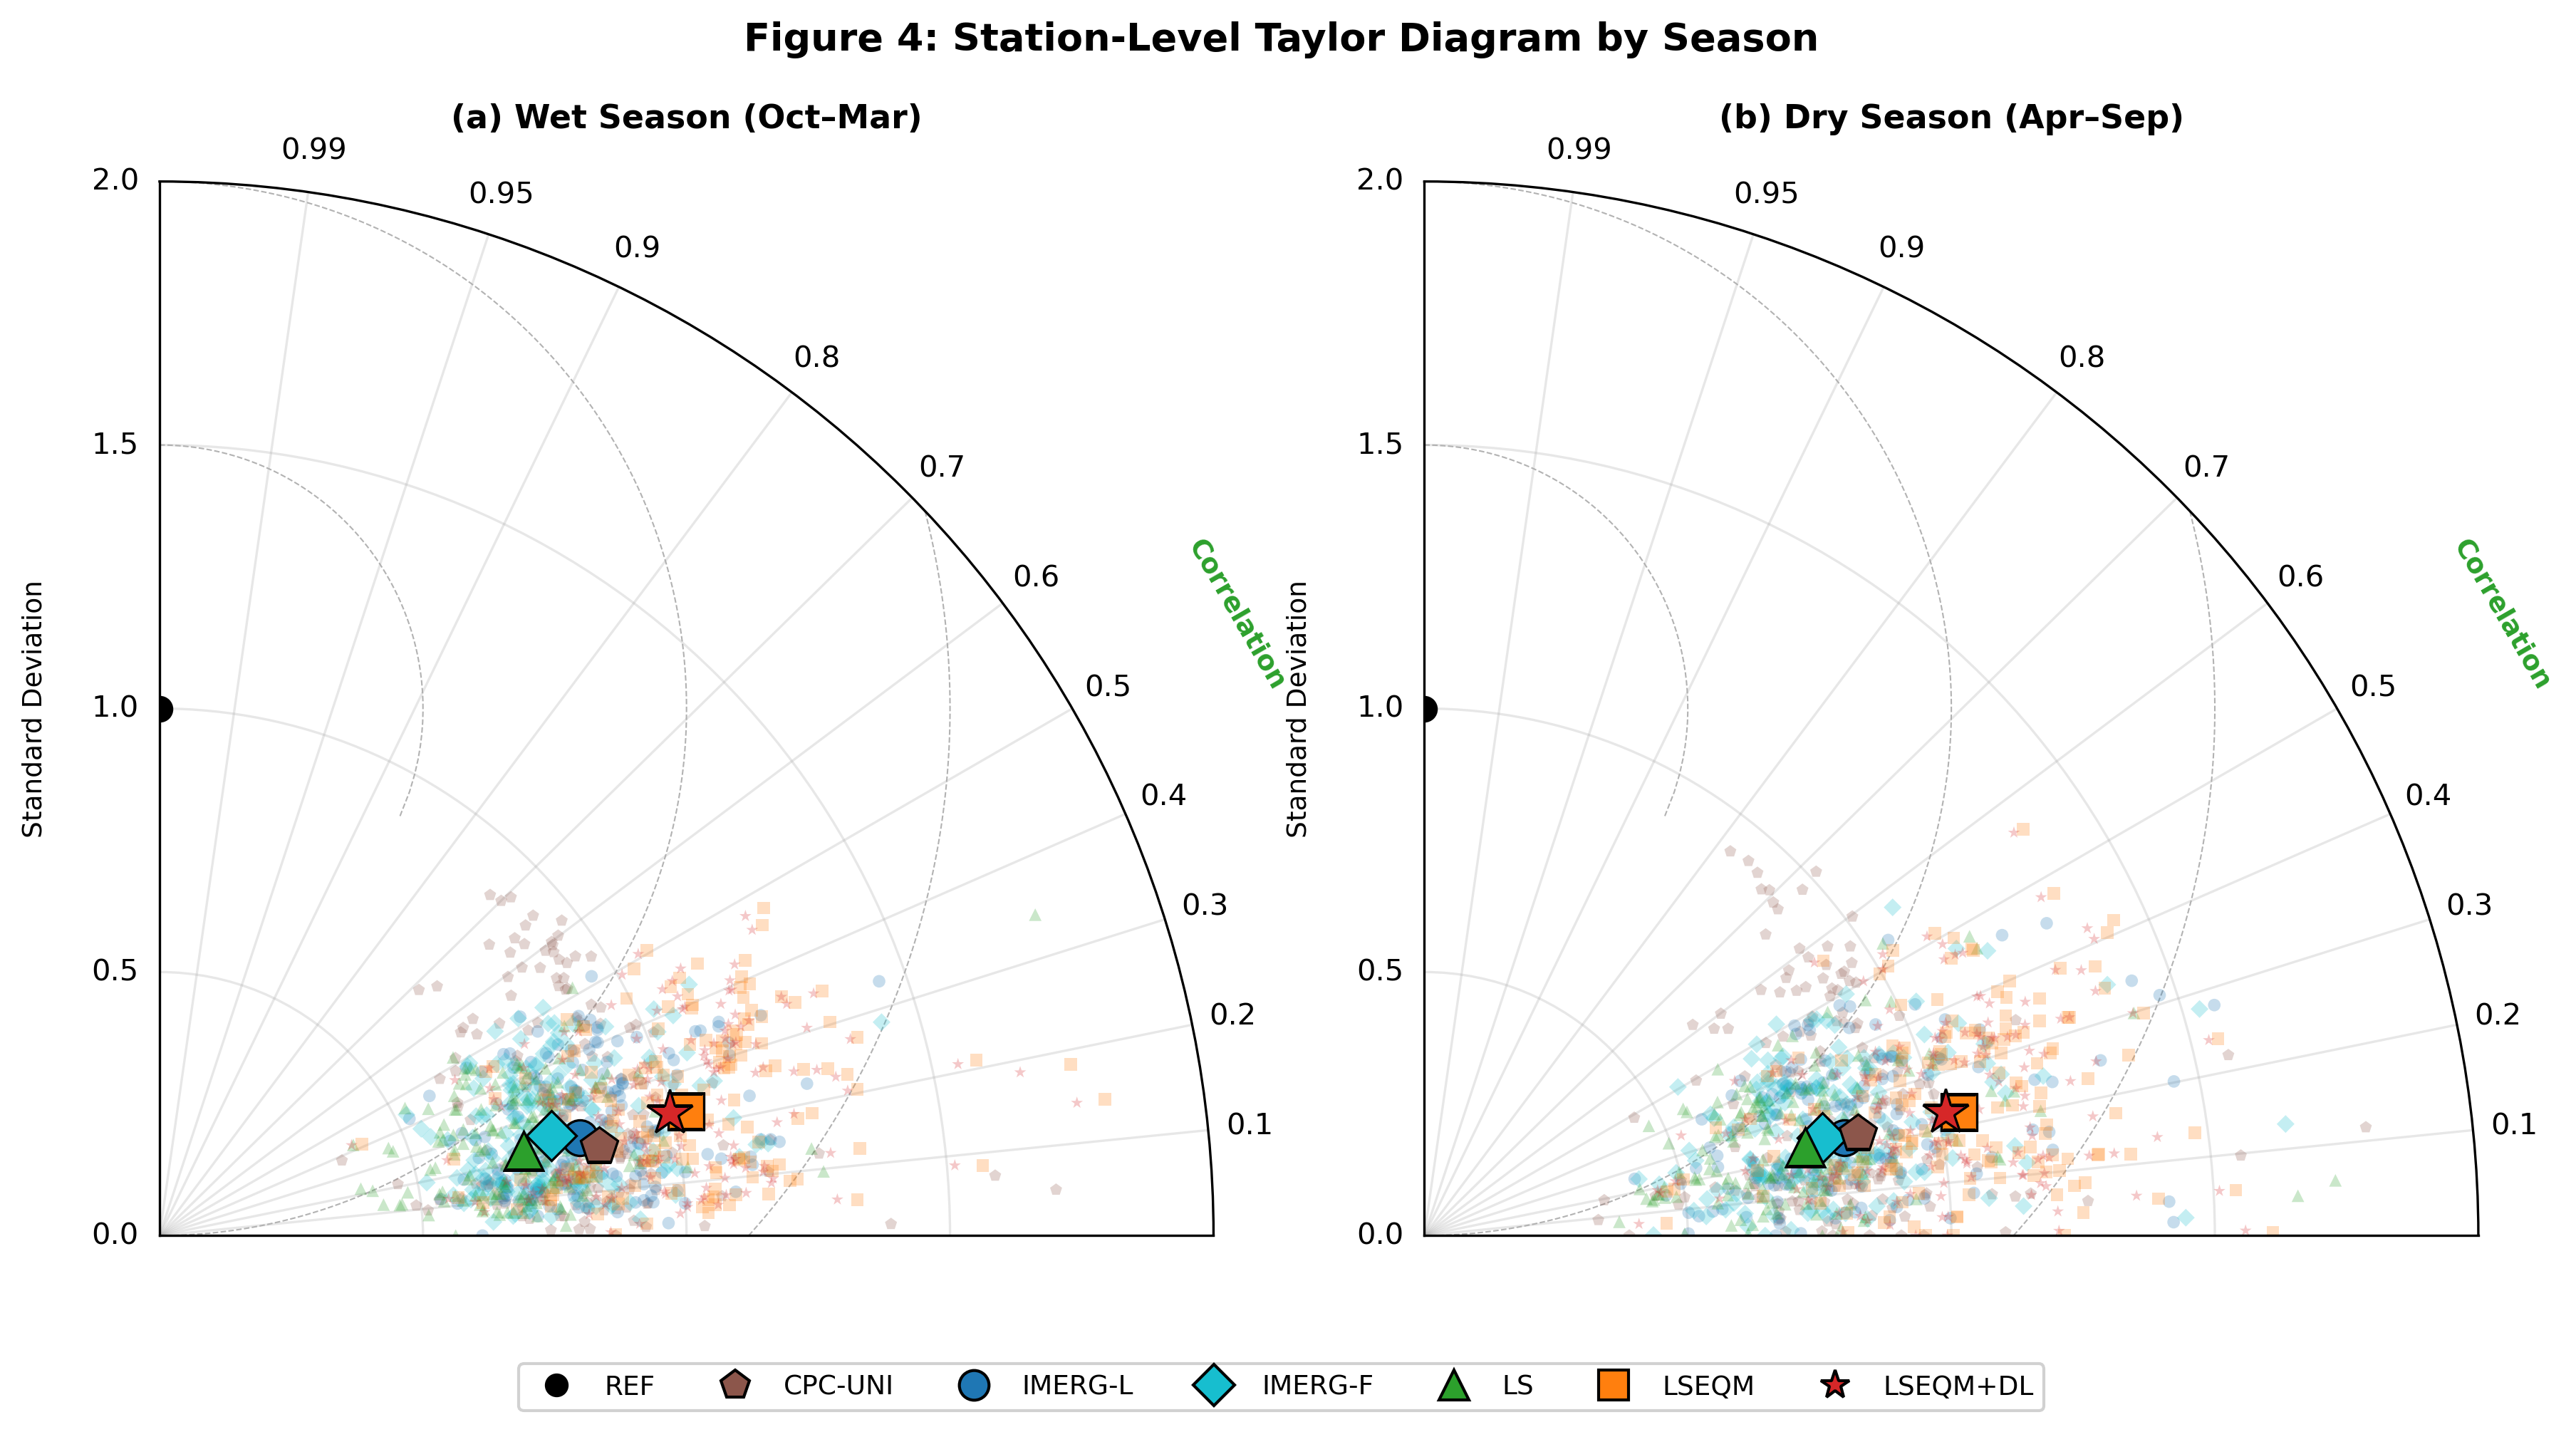
\includegraphics[width=\textwidth]{images/fig04_taylor_by_station.png}
\caption{Taylor diagrams comparing daily precipitation performance
against independent BMKG station observations, stratified by (a) wet
season (October--March) and (b) dry season (April--September). Products:
CPC-UNI (brown pentagon), IMERG-L (blue circle), IMERG-F (cyan diamond),
LS (green triangle), LSEQM (orange square), LSEQM+DL (red star). Large
markers show the per-station median; small translucent markers show
individual stations. Angular position: Pearson correlation; radial
distance: normalized standard deviation; gray arcs: centered RMSE
\cite{ref35}.\label{fig:taylor}}
\end{figure}

Figure~\ref{fig:taylor} provides a compact multi-dimensional summary of
correction performance against independent BMKG stations, stratified by
monsoon season. In both seasons, LS underestimates observed variability
(normalized standard deviation 0.71--0.74), while LSEQM and LSEQM+DL
bring the ratio toward unity (1.03/1.00 in the wet season,
1.04/1.02 in the dry season). Pearson correlation remains largely
unchanged across correction stages ($\approx$0.22--0.25), confirming
that distributional correction does not modify temporal prediction skill,
consistent with the theoretical expectation in Section~\ref{sec:domain}.
CPC-UNI itself does not coincide with the station reference point
(standard deviation ratio $\approx$0.85), reflecting interpolation
uncertainty at 0.5\textdegree{} resolution, a characteristic that
motivates the independent station validation in
Section~\ref{sec:station}.

\subsection{Independent Station Validation}\label{sec:station}

\begin{figure}[H]
\centering
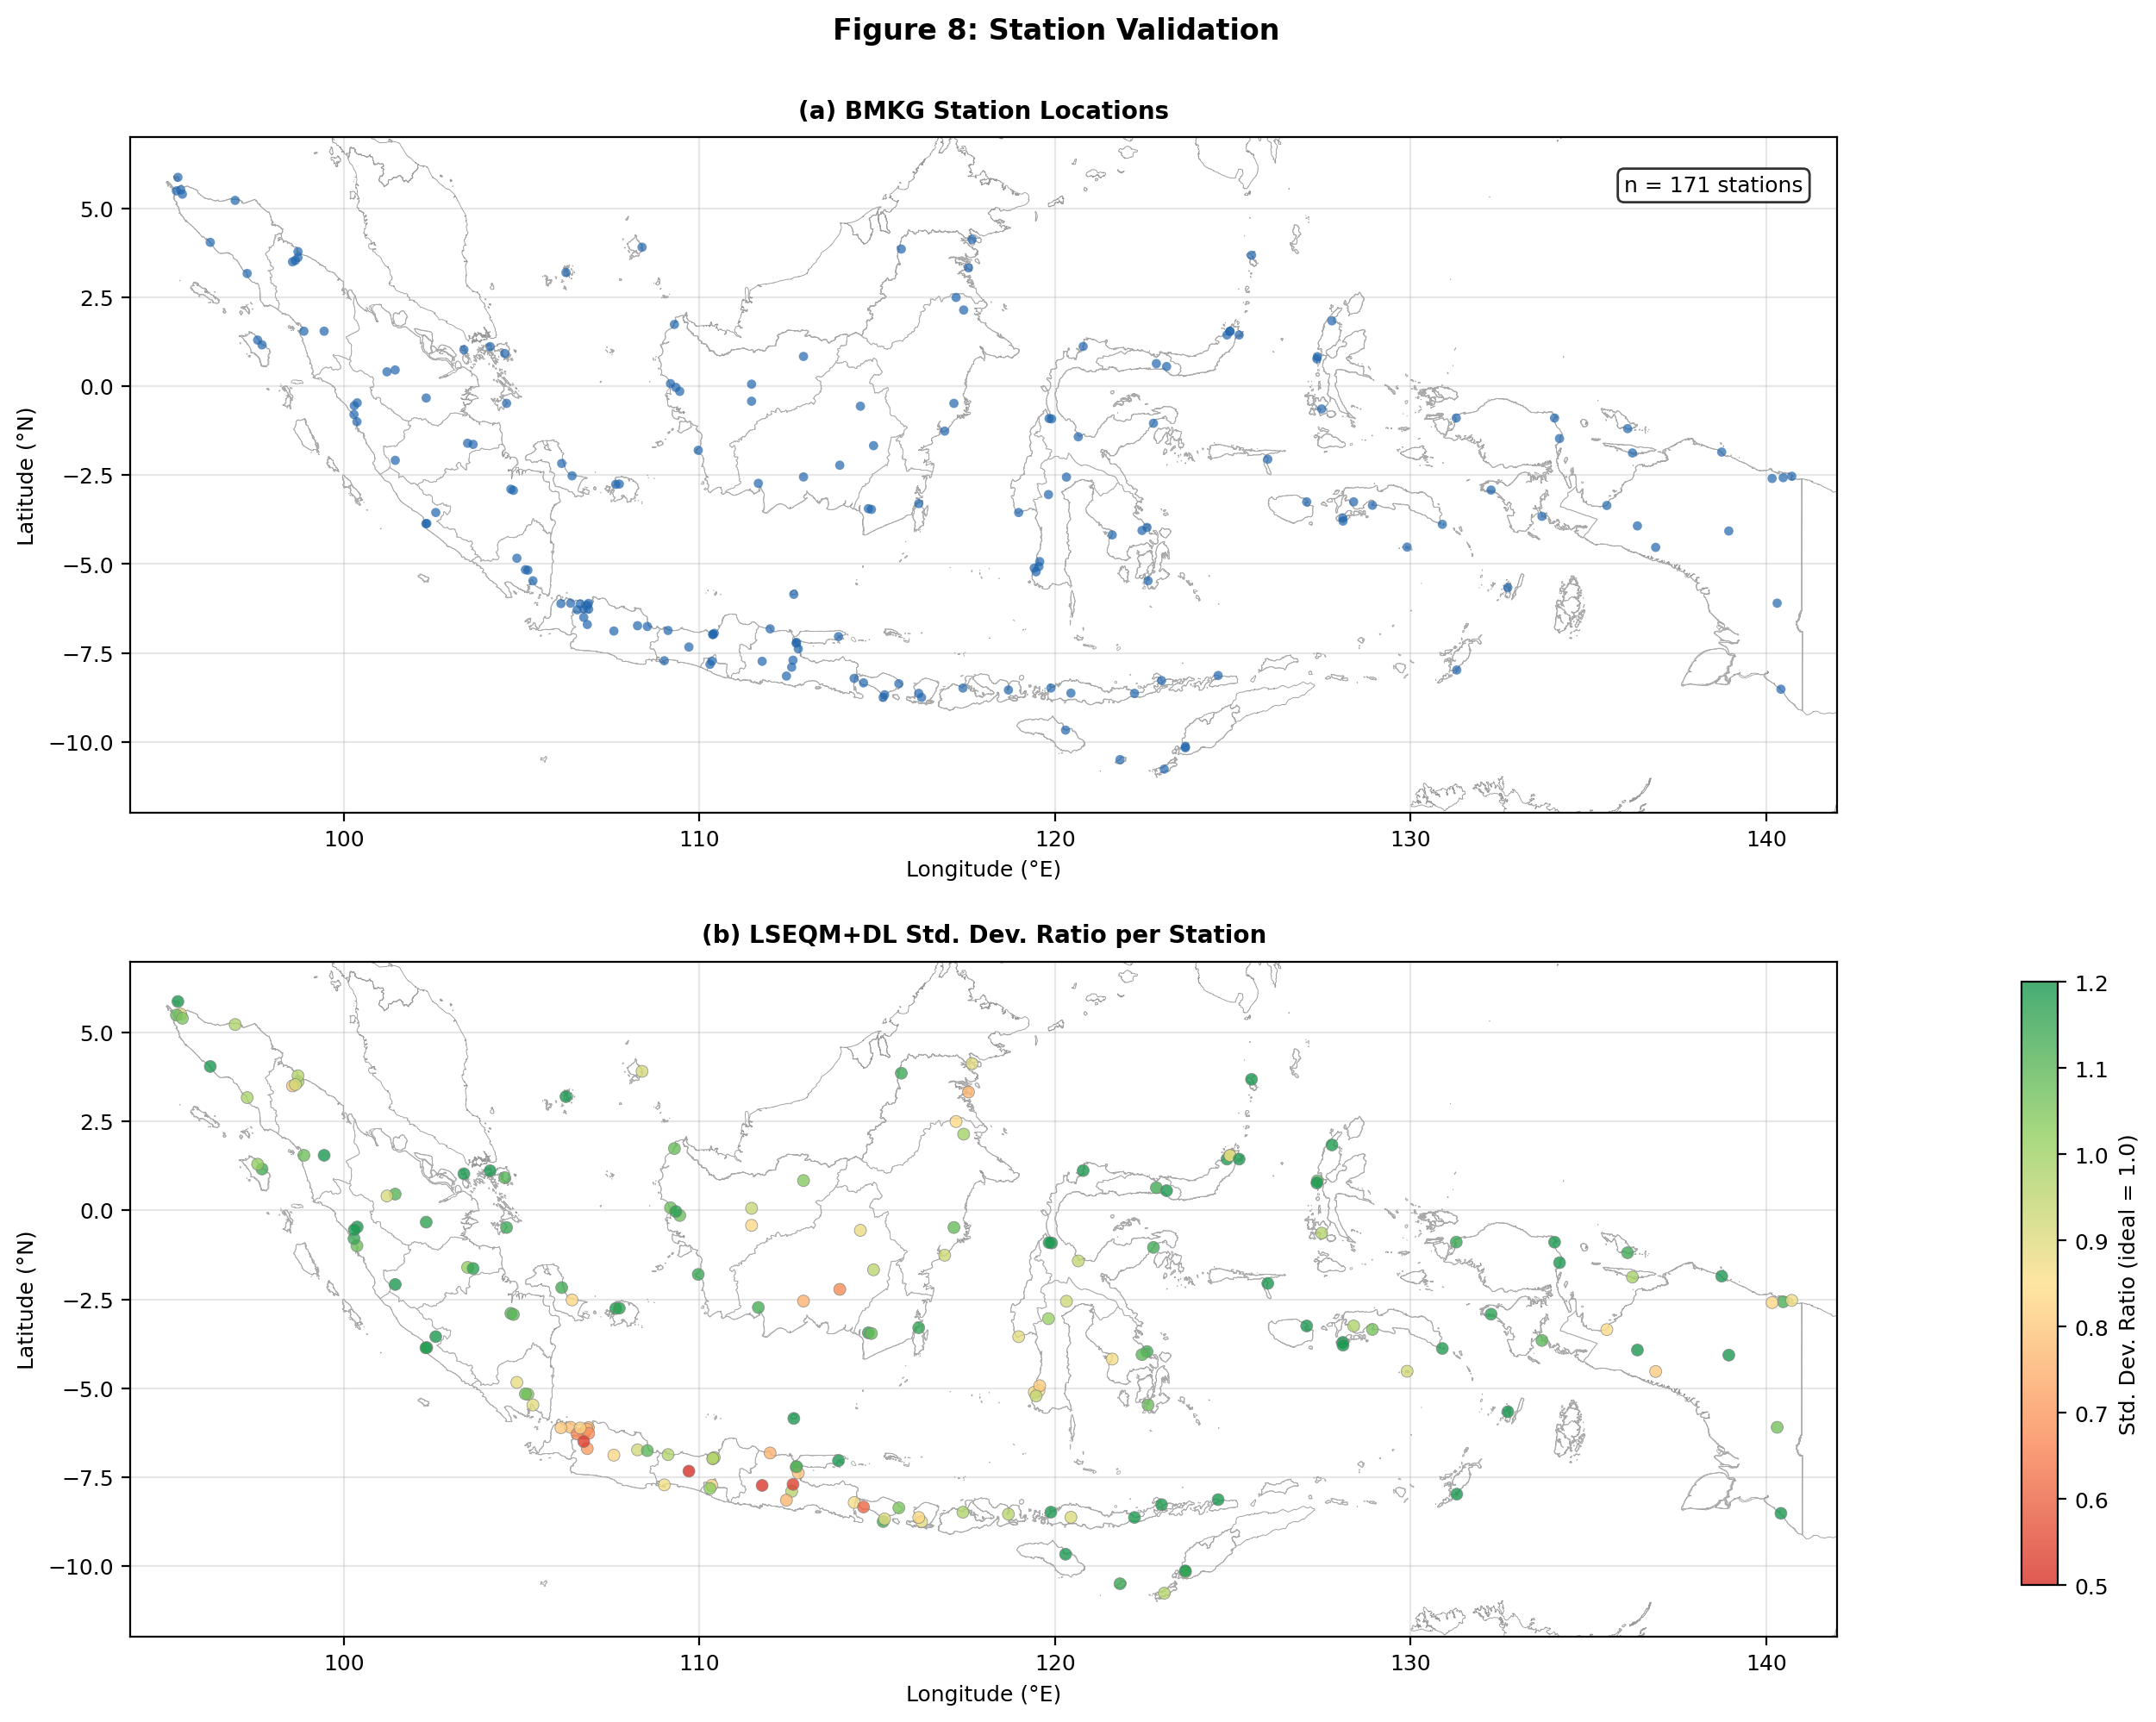
\includegraphics[width=0.75\textwidth]{images/fig08_station_validation.png}
\caption{(a) Location of the 171 BMKG stations used for independent
validation. (b) Per-station standard deviation ratio (LSEQM+DL
vs.\ observed), averaged across all dekadal periods. Values near 1.0
(green) indicate good variability preservation.\label{fig:stations}}
\end{figure}

Table~2 presents the median validation results across
171 BMKG stations. These observations are entirely independent of the
correction procedure and represent direct ground truth uncontaminated by
CPC-UNI interpolation uncertainty.

The LS-to-LSEQM transition delivers the largest improvements. The
standard deviation ratio moves from 0.71 to 1.03, correcting a 29\%
underestimation of precipitation variability to within 3\% of observed.
LSEQM+DL reaches 1.00 (exact match). The wet-day frequency ratio moves
from 1.21 to 0.96, reducing a 21\% overestimation of wet-day occurrence
to within 5\% of observed. The $Q_{99}$ ratio improves from 0.71 to 1.05
(LSEQM) and 1.01 (LSEQM+DL), recovering the large extreme rainfall
underestimation present in the LS product. The station-level relative
bias improves from $-$11.4\% to $-$0.6\%. These results confirm that the
apparent CPC-UNI overshoot in the domain-wide percentile ratios
(Section~\ref{sec:domain}) represents reference-side interpolation
uncertainty, not over-correction.

\phantomsection\label{tab:station}
\textbf{Table~2.} Independent station validation organized by the three
design objectives. Values represent the median across 171 BMKG stations
and all 36 dekadal periods. Ratio metrics express test/observed (target
= 1.0). Bold indicates the value closest to the target.

\begingroup\small
\begin{longtable}[]{@{}llllll@{}}
\toprule
Evaluation Objective & Metric & LS & LSEQM & LSEQM+DL & Target \\
\midrule
\endhead
\bottomrule
\endlastfoot
\textbf{Value Adjustment}
  & Relative Bias         & $-$0.114 & \textbf{0.009} & $-$0.006 & 0 \\
  & Std.\ Dev.\ Ratio     & 0.71 & 1.03 & \textbf{1.00} & 1.0 \\
\textbf{Distribution Alignment}
  & KS \(p\)-value (\%)   & 0.01 & \textbf{19.07} & \textbf{19.07} & 100 \\
  & Wet-Day Freq.\ Ratio  & 1.21 & \textbf{0.96} & 0.95 & 1.0 \\
  & Wet-Day Int.\ Ratio   & 0.71 & \textbf{1.06} & 1.05 & 1.0 \\
\textbf{Extreme Preservation}
  & \(Q_{95}\) Ratio      & 0.74 & \textbf{1.07} & 1.05 & 1.0 \\
  & \(Q_{99}\) Ratio      & 0.71 & 1.05 & \textbf{1.01} & 1.0 \\
\textbf{Event Detection}
  & POD                   & \textbf{0.78} & 0.65 & 0.65 & 1.0 \\
  & CSI                   & \textbf{0.53} & 0.49 & 0.49 & 1.0 \\
  & FAR                   & 0.36 & \textbf{0.32} & \textbf{0.32} & 0 \\
\end{longtable}
\endgroup

\subsection{Extreme Event Detection}\label{sec:extremes}

\begin{figure}[H]
\centering
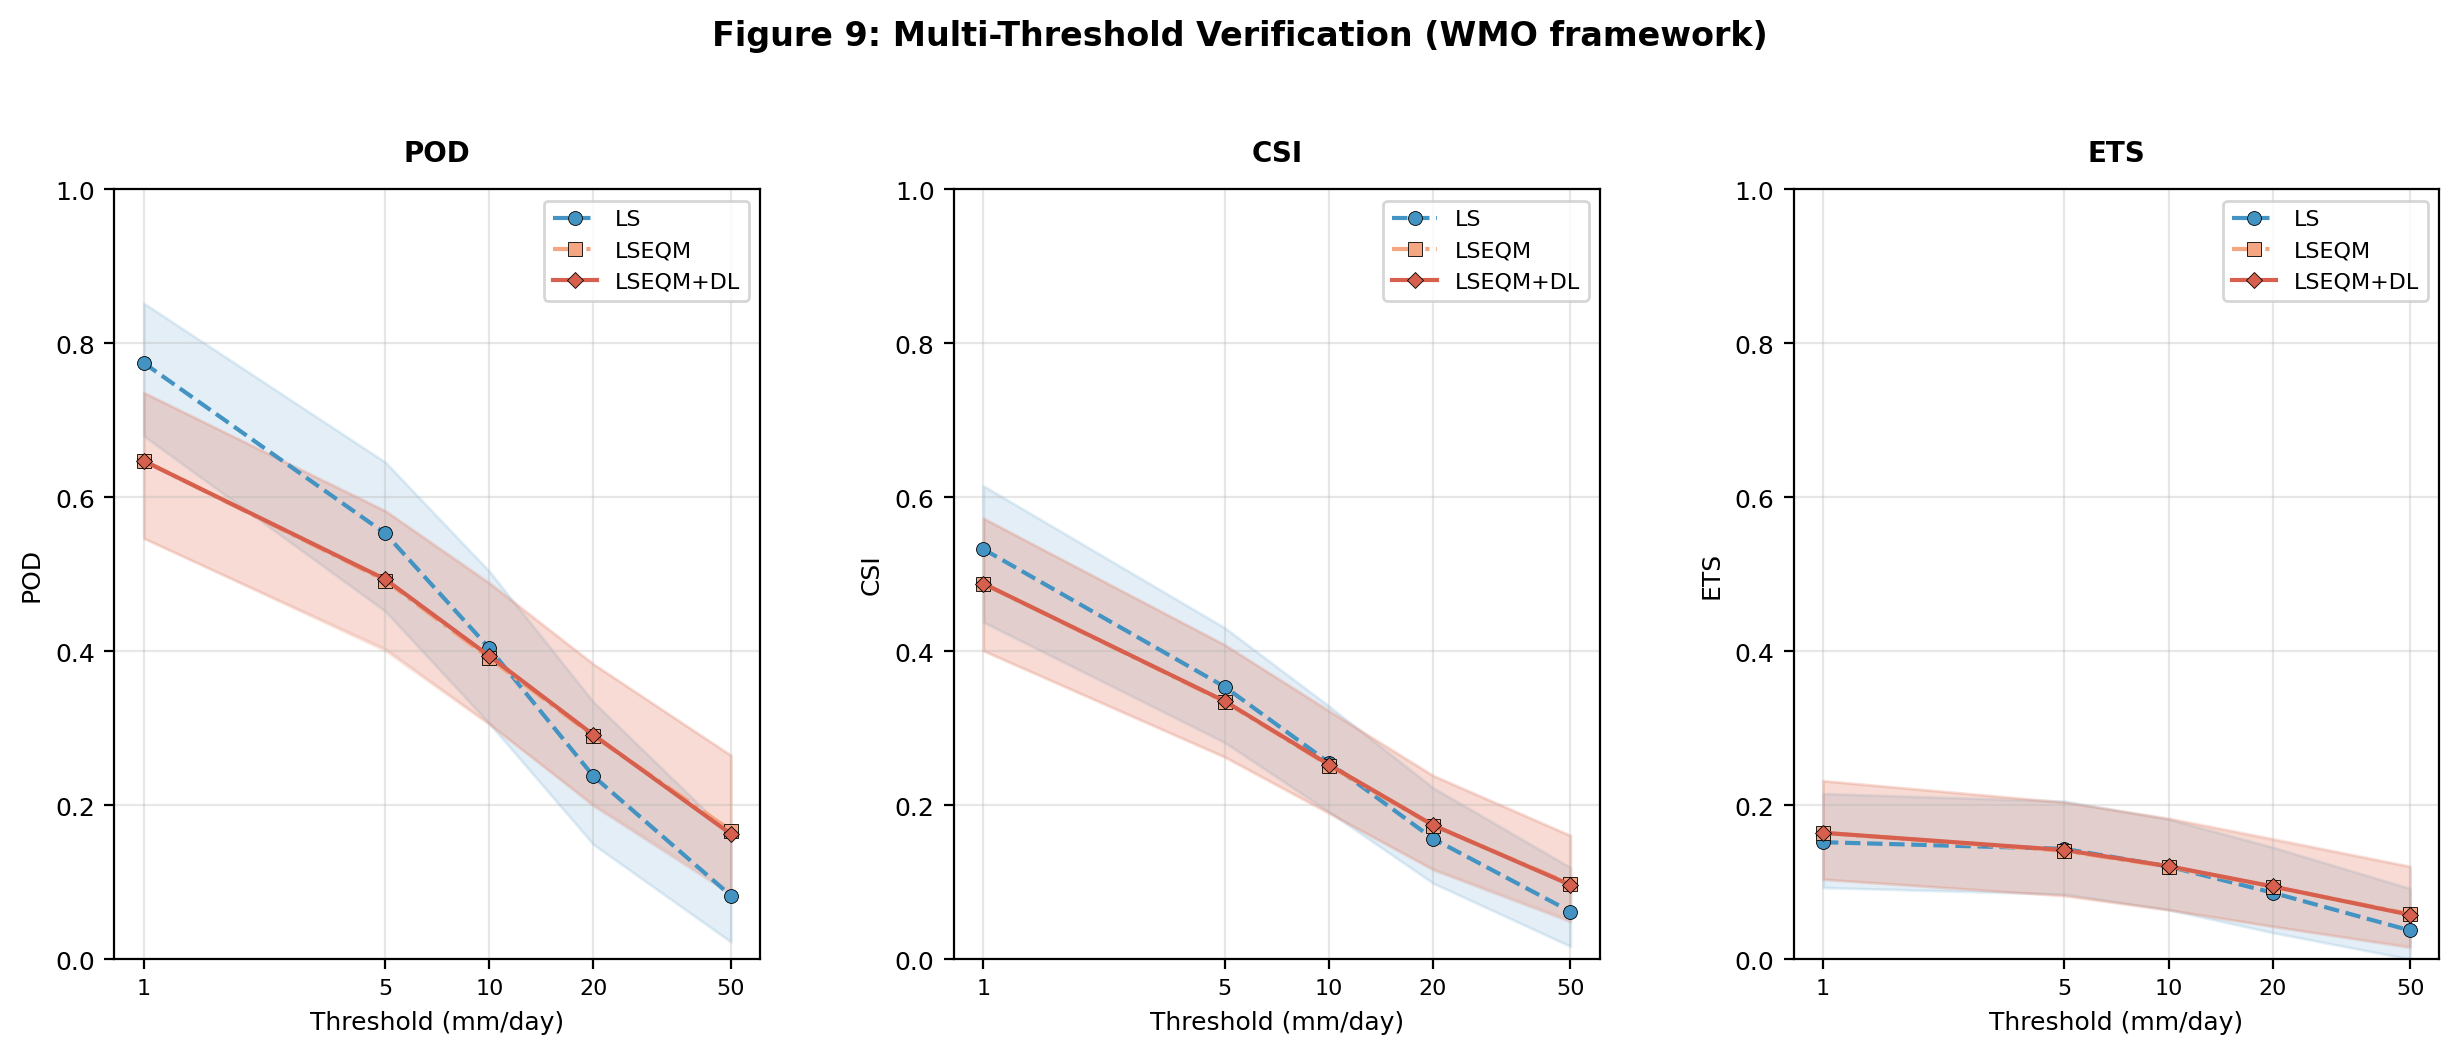
\includegraphics[width=\textwidth]{images/fig09_multi_threshold.png}
\caption{WMO multi-threshold verification at BMKG station locations:
(a) Probability of Detection (POD), (b) Critical Success Index (CSI),
and (c) Equitable Threat Score (ETS) as functions of precipitation
threshold for LS (blue), LSEQM (orange), and LSEQM+DL (green). Lines
show the station median; shading shows the interquartile range.
Thresholds: 1~mm (measurable), 5~mm (light), 10~mm (moderate), 20~mm
(moderate-heavy), 50~mm (heavy), 100~mm (very heavy), 150~mm
(extreme).\label{fig:threshold}}
\end{figure}

At the 1~mm threshold, LS achieves the highest POD (0.77) and CSI
(0.53), as the uniform multiplicative rescaling preserves the satellite
wet-day frequency. The pattern reverses above 20~mm/day: LSEQM and
LSEQM+DL maintain higher detection skill than LS at all higher
thresholds. At 50~mm, the median CSI for LSEQM+DL is 0.097 versus 0.062
for LS, a 57\% improvement. At 100~mm (very heavy rainfall), LSEQM+DL
achieves a median POD of 0.065 and CSI of 0.042, compared with 0.015
and 0.011 for LS. The Equitable Threat Score, which accounts for random
hits, shows the same pattern: at 50~mm, ETS for LSEQM+DL (0.058) exceeds
that of LS (0.038), confirming that the improved extreme detection is
not attributable to increased frequency bias.

\subsection{Temporal Stability}

\begin{figure}[H]
\centering
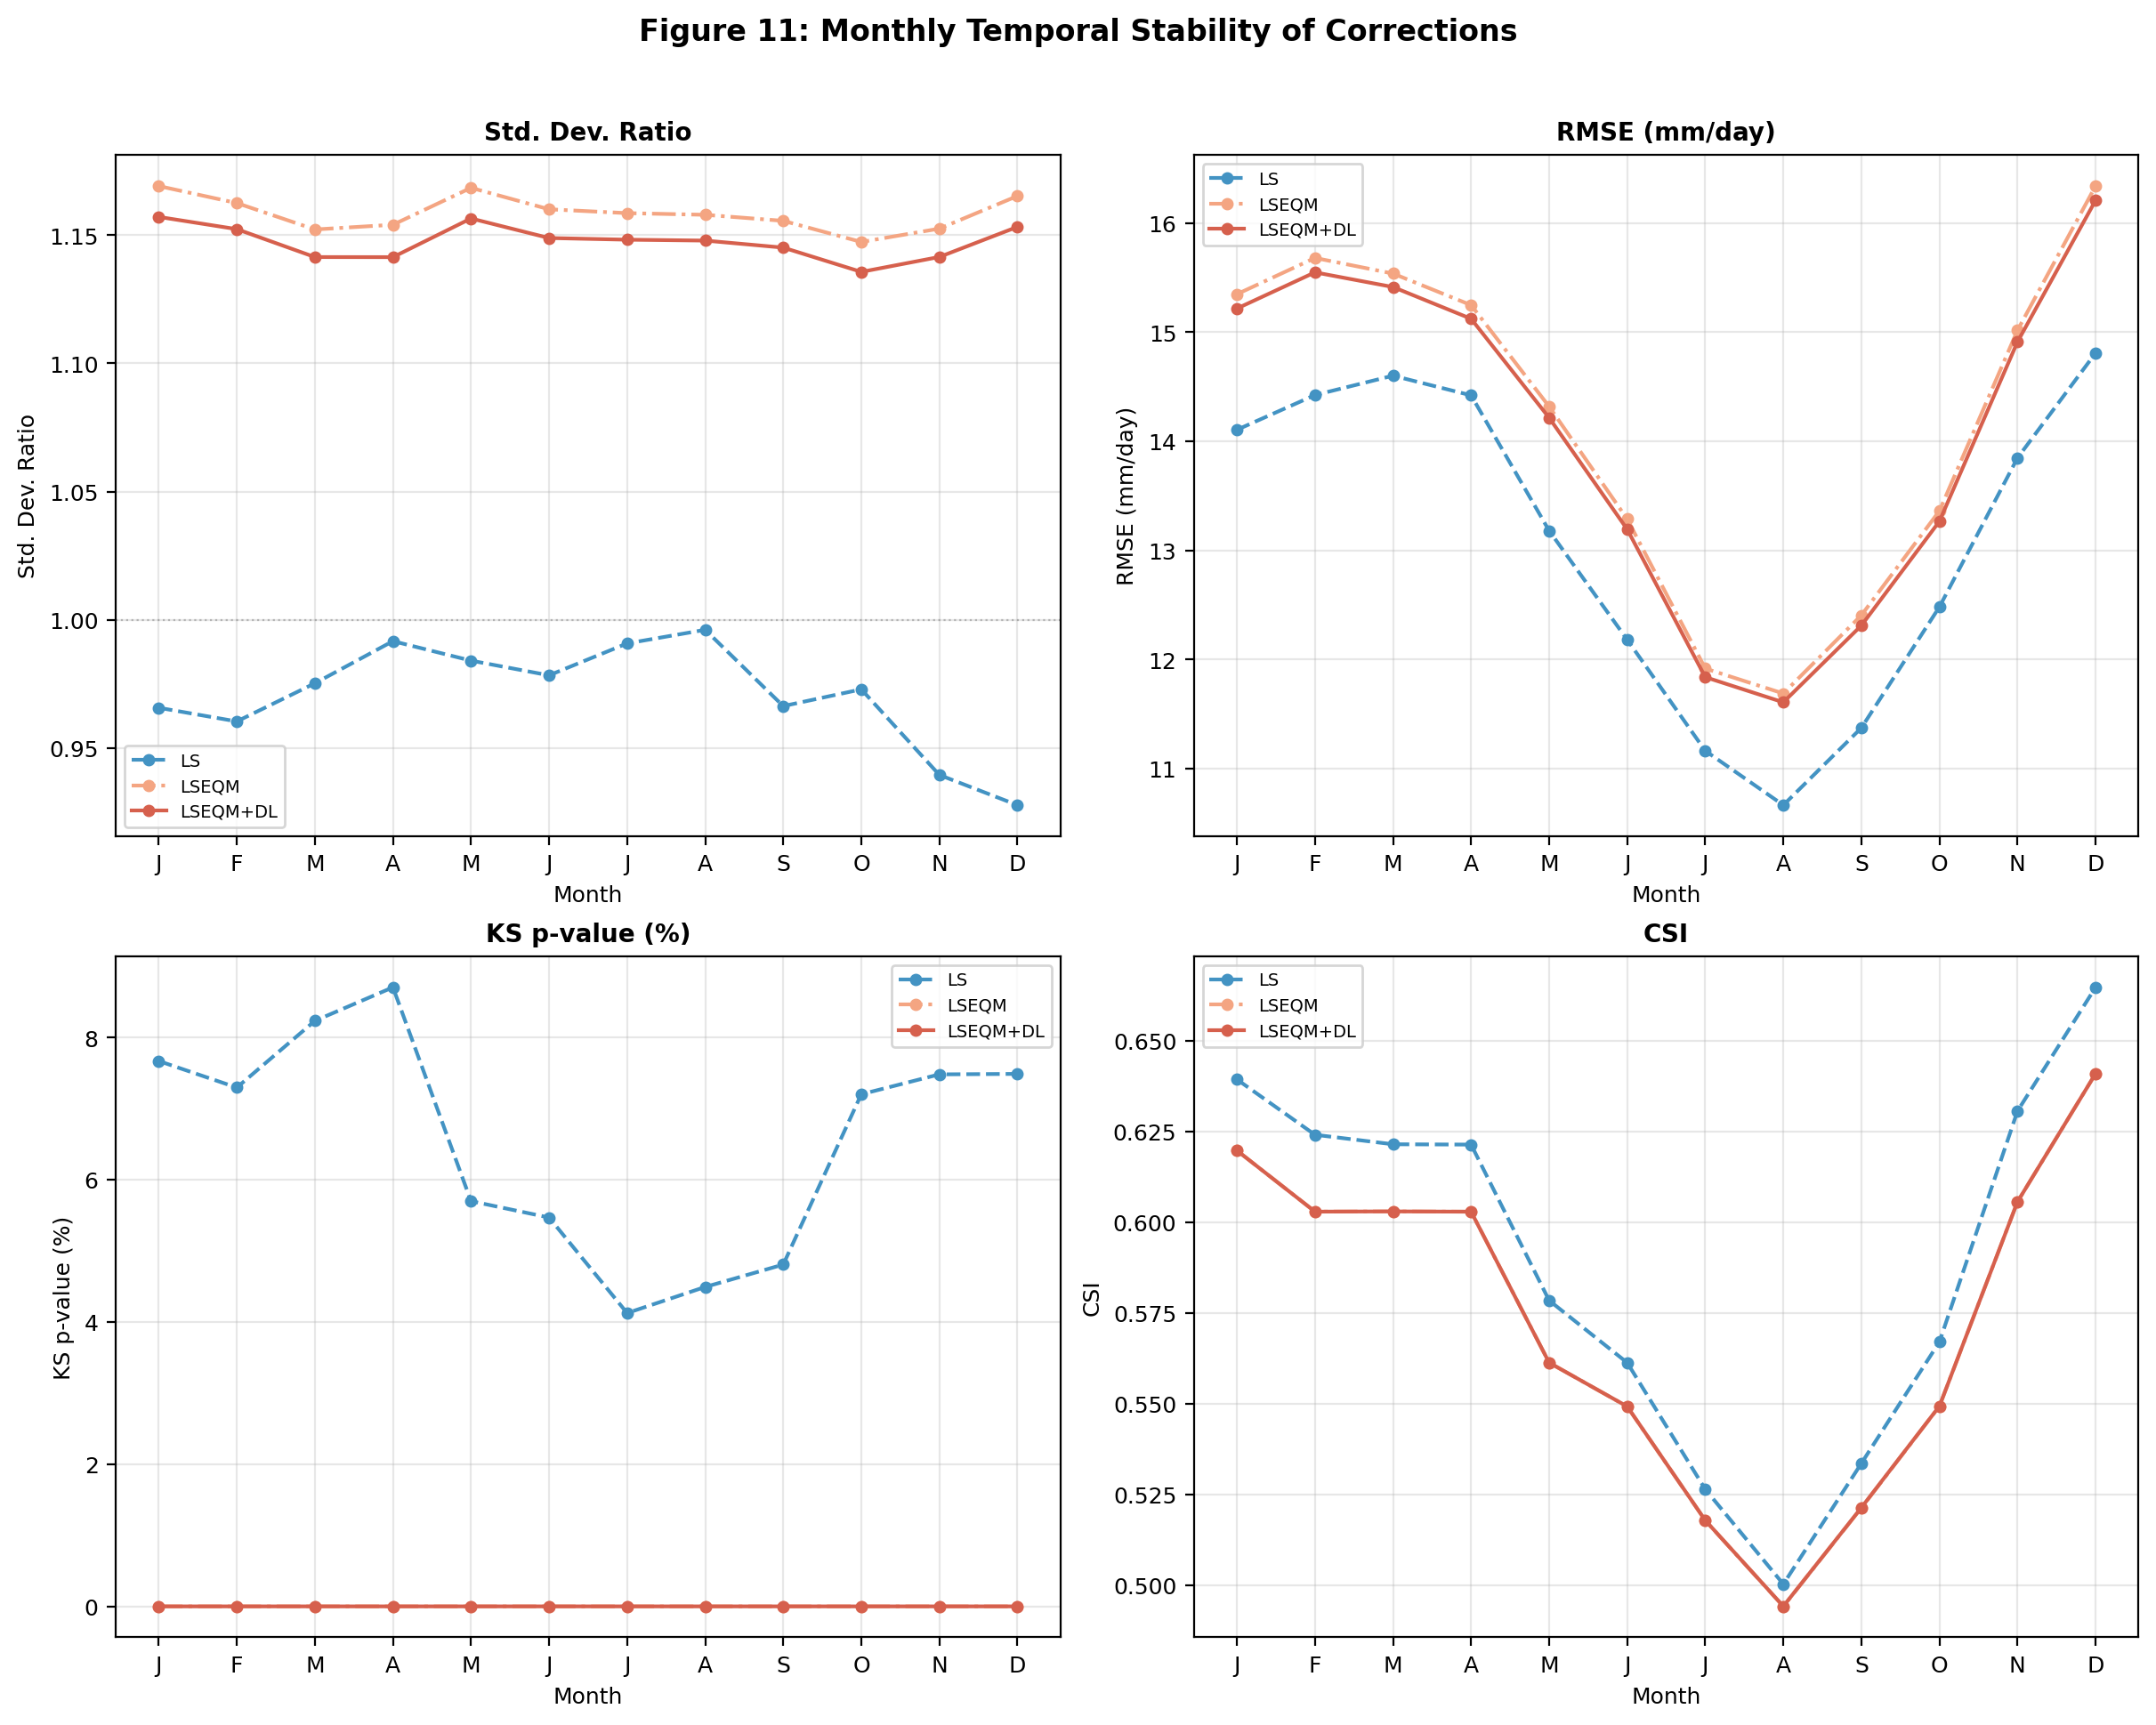
\includegraphics[width=\textwidth]{images/fig11_temporal_stability.png}
\caption{Monthly temporal stability of correction performance: (a)
standard deviation ratio, (b) RMSE (mm/day), (c) KS \(p\)-value (\%),
and (d) Critical Success Index (CSI). Lines show domain-median values
for LS (blue), LSEQM (orange), and LSEQM+DL (green). The seasonal cycle
reflects the wet (October--March) and dry (April--September) monsoon
regime.\label{fig:temporal}}
\end{figure}

Figure~\ref{fig:temporal} shows that the method ordering is stable
across all 12 calendar months and both monsoon regimes, with no
degradation during the wet season when precipitation intensities are
highest. The standard deviation ratio remains near 1.0 for LSEQM+DL
throughout the year, while LS consistently underestimates variability.
RMSE is higher for LSEQM and LSEQM+DL than LS, reflecting the wider
corrected distribution rather than degraded temporal accuracy.

% ============================================================
\section{Discussion and Conclusions}\label{discussion}

The LSEQM+DL framework delivers improvements across all three design
objectives, confirmed by independent validation against BMKG station
observations absent from the correction procedure. The staged design
assigns each component a specific role: LS removes the mean bias, EQM
with gamma fitting aligns the distribution body, GPD explicitly extends
the correction into the extreme tail, and CNN refinement addresses
spatially structured residuals in high-intensity pixels. The station
density confidence mask ensures that the CNN contribution is proportional
to the reliability of the training target.

Three findings warrant emphasis. First, the apparent overshoot of upper
percentile ratios against CPC-UNI resolves to near-unity at independent
stations (domain $Q_{99}$ ratio 1.196 vs.\ station $Q_{99}$ ratio 1.01),
supporting interpretation of the domain-wide residual as reference-side
interpolation uncertainty rather than over-correction. Second, the WMO
multi-threshold verification demonstrates that GPD tail adjustment
provides measurable skill above 20~mm/day that would be absent from a
pure EQM approach. Third, the trade-off between wet-day frequency
correction and event detection is explicit, predictable, and a direct
consequence of the dry-day frequency matching design \cite{ref11}, not an
uncontrolled artifact.

Several limitations apply. The blending weight ($\alpha = 0.70$) and
GPD threshold (80th percentile) were selected on domain expertise and
not formally optimized; formal sensitivity analysis is a priority for
future work. The CNN architecture is simple by design, given the limited
training sample ($\sim$250 values per dekad), and alternatives such as
U-Net may improve spatial refinement. No strict temporal hold-out is
applied, since per-dekad training pools all available years.

The framework relies on globally available datasets (IMERG, CPC-UNI)
and employs transferable statistical methods, supporting application to
other tropical and subtropical regions with sparse gauge networks.
Each correction stage targets a distinct, verifiable bias dimension,
making the framework modular: individual stages can be replaced or
recalibrated without redesigning the full pipeline. Ongoing work
targets additional Maritime Continent domains and formal evaluation of
the confidence mask sensitivity to the saturation count parameter.

% ============================================================
{\footnotesize
\begin{thebibliography}{47}

\bibitem{ref1} Hou, A.Y., Kakar, R.K., Neeck, S., Azarbarzin, A.A., Kummerow,
C.D., Kojima, M., Oki, R., Nakamura, K. and Iguchi, T. (2014). The
Global Precipitation Measurement Mission. \emph{Bull. Amer. Meteor.
Soc.}, 95(5), 701-722. DOI: 10.1175/BAMS-D-13-00164.1

\bibitem{ref2} Huffman, G.J., Bolvin, D.T., Braithwaite, D., Hsu, K.-L., Joyce,
R.J., Kidd, C., Nelkin, E.J., Sorooshian, S., Stocker, E.F., Tan, J.,
Wolff, D.B. and Xie, P. (2020). Integrated Multi-satellitE Retrievals
for the Global Precipitation Measurement (GPM) Mission (IMERG).
\emph{Satellite Precipitation Measurement}, Adv. Global Change Res., 67,
343-353. DOI: 10.1007/978-3-030-24568-9\_19

\bibitem{ref3} Maggioni, V., Meyers, P.C. and Robinson, M.D.~(2016). A Review
of Merged High-Resolution Satellite Precipitation Product Accuracy
during the Tropical Rainfall Measuring Mission (TRMM) Era. \emph{J.
Hydrometeor.}, 17(4), 1101-1117. DOI: 10.1175/JHM-D-15-0190.1

\bibitem{ref4} Teutschbein, C. and Seibert, J. (2012). Bias correction of
regional climate model simulations for hydrological climate-change
impact studies: Review and evaluation of different methods. \emph{J.
Hydrol.}, 456-457, 12-29. DOI: 10.1016/j.jhydrol.2012.05.052

\bibitem{ref5} Gudmundsson, L., Bremnes, J.B., Haugen, J.E. and Engen-Skaugen,
T. (2012). Technical Note: Downscaling RCM precipitation to the station
scale using statistical transformations -- a comparison of methods.
\emph{Hydrol. Earth Syst. Sci.}, 16, 3383-3390. DOI:
10.5194/hess-16-3383-2012

\bibitem{ref6} Themesssl, M.J., Gobiet, A. and Heinrich, G. (2012).
Empirical-statistical downscaling and error correction of regional
climate models and its impact on the climate change signal.
\emph{Climatic Change}, 112, 449-468. DOI: 10.1007/s10584-011-0224-4

\bibitem{ref7} Coles, S. (2001). \emph{An Introduction to Statistical Modeling
of Extreme Values}. Springer Series in Statistics. DOI:
10.1007/978-1-4471-3675-0

\bibitem{ref8} Maraun, D. (2016). Bias Correcting Climate Change Simulations --
a Critical Review. \emph{Curr. Clim. Change Rep.}, 2, 211-220. DOI:
10.1007/s40641-016-0050-x

\bibitem{ref9} Bano-Medina, J., Manzanas, R. and Gutierrez, J.M. (2020).
Configuration and intercomparison of deep learning neural models for
statistical downscaling. \emph{Geosci. Model Dev.}, 13, 2109-2124. DOI:
10.5194/gmd-13-2109-2020

\bibitem{ref10} Pan, B., Hsu, K., AghaKouchak, A. and Sorooshian, S. (2019).
Improving Precipitation Estimation Using Convolutional Neural Network.
\emph{Water Resour. Res.}, 55(3), 2301-2321. DOI: 10.1029/2018WR024090

\bibitem{ref11} Cannon, A.J., Sobie, S.R. and Murdock, T.Q. (2015). Bias
Correction of GCM Precipitation by Quantile Mapping: How Well Do Methods
Preserve Changes in Quantiles and Extremes? \emph{J. Climate}, 28(17),
6938-6959. DOI: 10.1175/JCLI-D-14-00754.1

\bibitem{ref12} Ehret, U., Zehe, E., Wulfmeyer, V., Warrach-Sagi, K. and
Liebert, J. (2012). HESS Opinions: Should we apply bias correction to
global and regional climate model data? \emph{Hydrol. Earth Syst. Sci.},
16, 3391-3404. DOI: 10.5194/hess-16-3391-2012

\bibitem{ref13} Chen, M., Shi, W., Xie, P., Silva, V.B.S., Kousky, V.E., Wayne
Higgins, R. and Janowiak, J.E. (2008). Assessing objective techniques
for gauge-based analyses of global daily precipitation. \emph{J.
Geophys. Res.}, 113, D04110. DOI: 10.1029/2007JD009132

\bibitem{ref14} Ebert, E.E. (2007). Methods for Verifying Satellite
Precipitation Estimates. \emph{Measuring Precipitation from Space}, Adv.
Global Change Res., 28, 345-356. DOI: 10.1007/978-1-4020-5835-6\_27

\bibitem{ref15} Wilks, D.S. (2011). \emph{Statistical Methods in the
Atmospheric Sciences}. 3rd ed.~Academic Press, International Geophysics
Series, Vol. 100. DOI: 10.1016/B978-0-12-385022-5.00001-4

\bibitem{ref16} Piani, C., Haerter, J.O. and Coppola, E. (2010). Statistical
bias correction for daily precipitation in regional climate models over
Europe. \emph{Theor. Appl. Climatol.}, 99, 187-192. DOI:
10.1007/s00704-009-0134-9

\bibitem{ref17} LeCun, Y., Bengio, Y. and Hinton, G. (2015). Deep learning.
\emph{Nature}, 521, 436-444. DOI: 10.1038/nature14539

\bibitem{ref18} Xie, P., Chen, M., Yang, S., Yatagai, A., Hayasaka, T.,
Fukushima, Y. and Liu, C. (2007). A Gauge-Based Analysis of Daily
Precipitation over East Asia. \emph{J. Hydrometeor.}, 8(3), 607-626.
DOI: 10.1175/JHM583.1

\bibitem{ref19} Aldrian, E. and Susanto, R.D. (2003). Identification of three
dominant rainfall regions within Indonesia and their relationship to sea
surface temperature. \emph{Int. J. Climatol.}, 23(12), 1435-1452. DOI:
10.1002/joc.950

\bibitem{ref20} As-syakur, A.R., Tanaka, T., Osawa, T. and Mahendra, M.S.
(2013). Indonesian rainfall variability observation using TRMM
multi-satellite data. \emph{Int. J. Remote Sens.}, 34(21), 7723-7738.
DOI: 10.1080/01431161.2013.826837

\bibitem{ref21} Pradhan, R.K., Markonis, Y., Varber, M.R., Franch, M.,
Papalexiou, S.M., Vidal, J.-P., Pappas, C., Hanel, M. and Hao, Z.
(2022). Review of GPM IMERG performance: A global perspective.
\emph{Remote Sens. Environ.}, 268, 112754. DOI:
10.1016/j.rse.2021.112754

\bibitem{ref22} Sun, Q., Miao, C., Duan, Q., Ashouri, H., Sorooshian, S. and
Hsu, K.-L. (2018). A Review of Global Precipitation Data Sets: Data
Sources, Estimation, and Intercomparisons. \emph{Rev.~Geophys.}, 56(1),
79-107. DOI: 10.1002/2017RG000574

\bibitem{ref23} Wood, A.W., Leung, L.R., Sridhar, V. and Lettenmaier, D.P.
(2004). Hydrologic implications of dynamical and statistical approaches
to downscaling climate model outputs. \emph{Climatic Change}, 62,
189-216. DOI: 10.1023/B:CLIM.0000013685.99609.9e

\bibitem{ref24} WMO (2008). \emph{Guide to Meteorological Instruments and
Methods of Observation}. WMO-No.~8, World Meteorological Organization,
Geneva.

\bibitem{ref25} Hosking, J.R.M. and Wallis, J.R. (1997). \emph{Regional
Frequency Analysis: An Approach Based on L-Moments}. Cambridge
University Press. DOI: 10.1017/CBO9780511529443

\bibitem{ref26} Kingma, D.P. and Ba, J. (2015). Adam: A Method for Stochastic
Optimization. \emph{Proc. 3rd Int. Conf. Learning Representations (ICLR
2015)}, San Diego.

\bibitem{ref27} Mega, T., Ushio, T., Matsuda, T., Kubota, T., Kachi, M. and
Oki, R. (2019). Gauge-Adjusted Global Satellite Mapping of
Precipitation. \emph{IEEE Trans. Geosci. Remote Sens.}, 57(4),
1928-1935. DOI: 10.1109/TGRS.2018.2870199

\bibitem{ref28} Nash, J.E. and Sutcliffe, J.V. (1970). River flow forecasting
through conceptual models part I -- A discussion of principles. \emph{J.
Hydrol.}, 10(3), 282-290. DOI: 10.1016/0022-1694(70)90255-6

\bibitem{ref29} Moriasi, D.N., Arnold, J.G., Van Liew, M.W., Bingner, R.L.,
Harmel, R.D. and Veith, T.L. (2007). Model evaluation guidelines for
systematic quantification of accuracy in watershed simulations.
\emph{Trans. ASABE}, 50(3), 885-900. DOI: 10.13031/2013.23153

\bibitem{ref30} Gupta, H.V., Kling, H., Yilmaz, K.K. and Martinez, G.F. (2009).
Decomposition of the mean squared error and NSE performance criteria:
Implications for improving hydrological modelling. \emph{J. Hydrol.},
377(1-2), 80-91. DOI: 10.1016/j.jhydrol.2009.08.003

\bibitem{ref31} Tan, J., Petersen, W.A. and Tokay, A. (2016). A Novel Approach
to Identify Sources of Errors in IMERG for GPM Ground Validation.
\emph{J. Hydrometeor.}, 17(9), 2477-2491. DOI: 10.1175/JHM-D-16-0079.1

\bibitem{ref32} Ramadhan, R., Yusnaini, H., Marzuki, M., Muharsyah, R.,
Suryanto, W., Sholihun, S., Vonnisa, M., Harmadi, H., Ningsih, A.P.,
Battaglia, A., Hashiguchi, H. and Tokay, A. (2022). Evaluation of GPM
IMERG Performance Using Gauge Data over Indonesian Maritime Continent at
Different Time Scales. \emph{Remote Sensing}, 14(5), 1172. DOI:
10.3390/rs14051172

\bibitem{ref33} Tang, G., Clark, M.P., Papalexiou, S.M., Ma, Z. and Hong, Y.
(2020). Have satellite precipitation products improved over last two
decades? A comprehensive comparison of GPM IMERG with nine satellite and
reanalysis datasets. \emph{Remote Sens. Environ.}, 240, 111697. DOI:
10.1016/j.rse.2020.111697

\bibitem{ref34} Maraun, D. (2013). Bias correction, quantile mapping, and
downscaling: Revisiting the inflation issue. \emph{J. Climate}, 26(6),
2137-2143. DOI: 10.1175/JCLI-D-12-00821.1

\bibitem{ref35} Taylor, K.E. (2001). Summarizing multiple aspects of model
performance in a single diagram. \emph{J. Geophys. Res.}, 106(D7),
7183-7192. DOI: 10.1029/2000JD900719

\bibitem{ref36} Adam, J.C. and Lettenmaier, D.P. (2003). Adjustment of global
gridded precipitation for systematic bias. \emph{J. Geophys. Res.},
108(D9), 4257. DOI: 10.1029/2002JD002499

\bibitem{ref37} Behrangi, A., Khakbaz, B., Jaw, T.C., AghaKouchak, A., Hsu, K.
and Sorooshian, S. (2011). Hydrologic evaluation of satellite
precipitation products over a mid-size basin. \emph{J. Hydrol.},
397(3-4), 225-237. DOI: 10.1016/j.jhydrol.2010.11.043

\bibitem{ref38} Rahmawati, N. and Lubczynski, M.W. (2018). Validation of
satellite daily rainfall estimates in complex terrain of Bali Island,
Indonesia. \emph{Theor. Appl. Climatol.}, 134(1--2), 513--532. DOI:
10.1007/s00704-017-2290-7

\bibitem{ref39} Wang, Z., Zhong, R., Lai, C. and Chen, J. (2017). Evaluation of
the GPM IMERG satellite-based precipitation products and the
hydrological utility. \emph{Atmos. Res.}, 196, 151-163. DOI:
10.1016/j.atmosres.2017.06.020

\bibitem{ref40} Sha, Y., Gagne II, D.J., West, G. and Stull, R. (2020).
Deep-learning-based gridded downscaling of surface meteorological
variables in complex terrain. Part I: Daily maximum and minimum 2-m
temperature. \emph{J. Appl. Meteor. Climatol.}, 59(12), 2057-2073. DOI:
10.1175/JAMC-D-20-0057.1

\bibitem{ref41} Vandal, T., Kodra, E., Ganguly, S., Michaelis, A., Nemani, R.
and Ganguly, A.R. (2017). DeepSD: Generating high fidelity daily climate
surfaces with generative adversarial networks. \emph{Proc. 23rd ACM
SIGKDD Int. Conf. on Knowledge Discovery and Data Mining}, 1375-1383.
DOI: 10.1145/3097983.3098004

\bibitem{ref42} Beck, H.E., Wood, E.F., Pan, M., Fisher, C.K., Miralles, D.G.,
van Dijk, A.I.J.M., McVicar, T.R. and Adler, R.F. (2019). MSWEP V2
Global 3-Hourly 0.1 degrees Precipitation: Methodology and Quantitative
Assessment. \emph{Bull. Amer. Meteor. Soc.}, 100(3), 473-500. DOI:
10.1175/BAMS-D-17-0138.1

\bibitem{ref43} Lange, S. (2019). Trend-preserving bias adjustment and
statistical downscaling with ISIMIP3BASD (v1.0). \emph{Geosci. Model
Dev.}, 12, 3055-3070. DOI: 10.5194/gmd-12-3055-2019

\bibitem{ref44} Hempel, S., Frieler, K., Warszawski, L., Schewe, J. and
Piontek, F. (2013). A trend-preserving bias correction -- the ISI-MIP
approach. \emph{Earth Syst. Dynam.}, 4, 219-236. DOI:
10.5194/esd-4-219-2013

\bibitem{ref45} Baez-Villanueva, O.M., Zambrano-Bigiarini, M., Beck, H.E.,
McNamara, I., Ribbe, L., Nauditt, A., Birkel, C., Verbist, K.,
Giraldo-Osorio, J.D. and Thinh, N.X. (2020). RF-MEP: A novel Random
Forest method for merging gridded precipitation products and
ground-based measurements. \emph{Remote Sens. Environ.}, 239, 111606.
DOI: 10.1016/j.rse.2019.111606

\bibitem{ref46} Sillmann, J., Kharin, V.V., Zhang, X., Zwiers, F.W. and
Bronaugh, D. (2013). Climate extremes indices in the CMIP5 multimodel
ensemble: Part 1. Model evaluation in the present climate. \emph{J.
Geophys. Res. Atmos.}, 118, 1716-1733. DOI: 10.1002/jgrd.50203

\bibitem{ref47} Wu, P., Yamanaka, M.D.~and Matsumoto, J. (2008). The Formation
of Nocturnal Rainfall Offshore from Convection over Western Kalimantan
(Borneo) Island. \emph{J. Meteor. Soc. Japan}, 86A, 187-203. DOI:
10.2151/jmsj.86A.187

\end{thebibliography}
}

\end{document}
